\documentclass[12pt, titlepage]{article}
\usepackage[utf8]{inputenc}
\usepackage[ngerman]{babel}
\usepackage{graphicx}
\usepackage[a4paper,lmargin={2cm},rmargin={2cm},
tmargin={2.5cm},bmargin = {2.5cm}]{geometry}
\usepackage{hyperref}
\usepackage{listings}
\usepackage{color}
\usepackage{caption}
\hypersetup{
    colorlinks,
    citecolor=black,
    filecolor=black,
    linkcolor=black,
    urlcolor=blue
}
\lstloadlanguages{csh}
\lstset{
language=csh,
basicstyle=\footnotesize\ttfamily,
numbers=left,
numberstyle=\tiny,
numbersep=5pt,
tabsize=2,
extendedchars=true,
breaklines=true,
frame=b,
stringstyle=\color{blue}\ttfamily,
showspaces=false,
showtabs=false,
xleftmargin=17pt,
framexleftmargin=17pt,
framexrightmargin=5pt,
framexbottommargin=4pt,
commentstyle=\color{green},
morecomment=[l]{//}, %use comment-line-style!
morecomment=[s]{/*}{*/}, %for multiline comments
showstringspaces=false,
morekeywords={ abstract, event, new, struct,
as, explicit, null, switch,
base, extern, object, this,
bool, false, operator, throw,
break, finally, out, true,
byte, fixed, override, try,
case, float, int2, params, typeof,
catch, for, private, uint,
char, foreach, protected, ulong,
checked, goto, public, unchecked,
class, if, readonly, unsafe,
const, implicit, ref, ushort,
continue, in, return, using,
decimal, int, sbyte, virtual,
default, interface, sealed, volatile,
delegate, internal, short, void,
do, is, sizeof, while,
double, lock, stackalloc,
else, long, static,
enum, namespace, string},
keywordstyle=\color{cyan},
identifierstyle=\color{red},
backgroundcolor=\color{cloudwhite},
}

\linespread{1.5}

\definecolor{red}{rgb}{0.6,0,0} 
\definecolor{blue}{rgb}{0,0,0.6}
\definecolor{green}{rgb}{0,0.8,0}
\definecolor{cyan}{rgb}{0.0,0.6,0.6}
\definecolor{cloudwhite}{rgb}{0.9412, 0.9608, 0.8471}

%Variablen
\newcommand{\myTitle}{Unity ECS}

\begin{document}
\begin{titlepage}
\centering
{\huge Friedrich-Schiller-Universität Jena \par}
{\large Fakultät für Mathematik und Informatik\par}
\vspace{1.5cm}
{\huge\bfseries \myTitle\par}
\vspace{2cm}
{\Large Bachelorarbeit zur Erlangung des akademischen Grades\\Bachelor of Science (B.Sc.) \par}
\vspace{3cm}
{\large vorgelegt von Dennis Untiet\\Matrikelnummer: 192151\par}
\vspace{0.5cm}
{\large geboren am 01.10.2001\quad in Esslingen\par}
\vspace{2cm}
{\large Erstgutachter*in:\\Zweitgutachter*in:\par} 
\vfill
{\Large Jena, \today}
\end{titlepage}
\section{Kurzfassung}
In der Bachelorarbeit über {\myTitle} geht es um Daten-orientierte Programmierung. Insbesondere wird das Entity Component System von Unity betrachtet.
\newpage
\tableofcontents
\newpage
\section{Einleitung}
\newpage
\section{Datenorientierte Programmierung}
\subsection{Was ist das Datenorientierte Design?}
Data-Oriented Design \cite{Data-OrientedDesign}\\
Probleme mit OOP: Hauptspeicher Zugriff und Cache misses. Versuche Code zu Parallelisieren sind zu viel Aufwand und bringen kaum etwas. Code ist sehr komplex.\\Datenorientiertes Design ist ein anderer Ansatz, der diese Probleme zu lösen versucht. Datenorientierung ändert die Sichtweise des Programmierens: Weg von Objekten, hin zu den eigentlichen Daten, wie diese im Speicher liegen und wie sie gelesen und verändert werden. Beim Programmieren geht es immer um das Verändern von Daten. Es ist die Beschreibung wie aus eingegebenen Daten veränderte Daten werden. Daher ergibt es Sinn sich direkt mit den Daten zu befassen. Zusätzlich: \glqq data-oriented design\grqq{}  hat nichts mit \glqq data-driven\grqq{} zu tun.\\ Ideale Daten:\\Kommt auf die Daten an und wie sie genutzt werden. Am besten wenn man die Daten mit möglichst geringem Aufwand nutzen kann. Also kleinstmögliche Veränderung. Das Programms wird um die ideale Datenstruktur gebaut.\\Objekte sind oft wie Bäume gebaut. Objekte interagieren oft mit anderen Objekte \glqq unter\grqq{} ihnen. Iteriert man über eine Anzahl an Objekten passiert das mehrfach mit beliebigen Objekten. Für ein Ideales Layout sollte ein Objekt in Komponenten zerlegt werden. Komponenten der gleichen Art können dann als Gruppe zusammen im Speicher liegen, egal von welchem Objekt sie kommen. Daraus resultierten große Gruppe homogener Daten, welche dann sequenziell verarbeitet werden können.\\Vorteile:\\Parallelisierung: Die Daten können sehr leicht auf mehrere Threads aufgeteilt werden ohne großen Aufwand\\Cache Affinität: Sehr Effizient, da der selbe Code immer wieder ausgeführt wird. Wenn die Daten sequenziell verarbeitet werden resultiert das in sehr guter Performance und fast perfekter Cache Nutzung.\\Modularität: Wenn Code zur Verbesserung der Performance angepasst wird, resultiert das oft in schlechter lesbarem und schlechter wartbarem Code. Bei Konzentration auf die Transformierung der Daten hat man am Ende kleinere Funktionen mit weniger Abhängigkeiten.\\Testing: Unit Test für Objektinteraktionen können kompliziert sein. Im Datenorientierten Design sind Unit Tests jedoch sehr einfach. Eingabe Daten erstellen, Funktion aufrufen und die Ausgabedaten verifizieren.\\Nachteile: Nicht die Lösung für alles. Schwierig zu lernen, da es ganz anders ist. Auch schwierig mit bestehendem prozedurale / Objektorientiertem Code zu verbinden.\\Anwendung: Klassifizierung, wie Daten genutzt werden: read-only / read-write / write-only. Welche Daten werden von dem System gebraucht? Nicht wie verhält sich ein Gegner sonder eher wie sich alle verhalten.\\Platz für OOP?: Teils / teils. Für einzelne Objekte (beispielsweise GUI) kann es sinnvoll sein. Sollte aber dennoch Datenorientiert geschrieben werden.
\\ DOD \cite{DOD}\\
Datenorientiertes Design kann auch mit anderen Programmier Paradigmen co-existieren. Datenorientierung wird mehr gebraucht, da Spiele immer komplexer werden und die Abstraktion durch OOP das Bottleneck sein wird. Überall sind Daten: Graphik auf dem Bildschirm, Positionen und Bewegung von Partikeln und so weiter. All diese Daten müssen auf etwas laufen, sei es eine VM oder etwas konkretes wie der CPU oder der GPU. Diese Daten existieren auf der Hardware irgendwo. Datenorientiertes Design ist das designen von Software, welche Transformationen auf wohldefinierten Daten ausführt. \\
Beispiel:
\subsection{Umsetzung Datenorientierter Programmierung}
\newpage
\section{Unity's Datenorientierter Technologie-Stack}
Die gesamte Bachelorarbeit wurde mit der Unity Entities Version 1.0.0-pre.65 verfasst. Dies ist Stand 01.04.2023 die aktuellste Version von Unity's Enitity Component System.\\
\href{https://unity.com/de/dots}{DOTS Homepage} \\
Unity's Datenorientierter Ansatz ist Unity's Datenorientierter Technologie-Stack. Dieser besteht aus 3 Teilen:\\
1. Das Entity Component System (ECS) für Unity. Dies ist ein Daten-orientierter Framework für Unity. Dieser ist auch kompatibel mit GameObjects, was Unity's üblicher Objektorientierter Ansatz ist.\\2. Der Burst Compiler. Der Burst Compiler übersetzt von IL/.NET Bytecode zu optimierten nativen Code. Es nutzt die LLVM Compiler Infrastruktur.\\3. Das C\# Job System. Das Job System von Unity erlaubt parallelen Code zu schreiben, welcher sicher und schnell läuft.
\subsection{Entity Component System}
\subsubsection{Entities}
\href{https://docs.unity3d.com/Packages/com.unity.entities@1.0/manual/concepts-entities.html}{Entity Dokumentation}\\Entities repräsentieren Dinge in dem Spiel. Sie besitzen weder Daten noch ein Verhalten, sondern zeigen lediglich auf, welche Daten zusammengehören. \\Der Entitymanager managt alle Entites in einer World \href{https://docs.unity3d.com/Packages/com.unity.entities@0.1/manual/world.html}{World Dokumentation}. In dem Entitymanager sind alle Entities gespeichert und er organisiert die Daten, welche mit einem Entity in Verbindung stehen. 
\subsubsection{Components}
\href{https://docs.unity3d.com/Packages/com.unity.entities@1.0/manual/concepts-components.html}{Components Dokumentation}\\Components repräsentieren die Daten des Spiels. Components speichern die Daten eines Entity. Diese Daten werden von System genutzt und verarbeitet. Dabei unterscheidet man zwischen verwalteten Components und unverwalteten Components. Unverwaltete Components sind in Unity C\# Strukturen, also leichtgewichtiger als Klassen. Diese können auch nur unverwaltete Daten speichern. Verwaltete Components werden hingegen als Klassen definiert und können alle Daten halten. Es ist jedoch üblich Strukturen zu verwenden, da diese mehr Performance bieten. Um ein unverwaltetes Component zu erstellen kann man das IComponentData Interface verwenden. Ein einfaches Component könnte also wie folgt aussehen:\begin{lstlisting}[language={[Sharp]C}, caption={Component example}]
using Unity.Entities;
using Unity.Mathematics;

namespace ECS.Components
{
    public struct ComponentExample : IComponentData
    {
        public int2 position;
        public float speed;
    }
}
\end{lstlisting}
Es gibt aber auch andere Arten von Components. 
\subsubsection{Systems}
\href{https://docs.unity3d.com/Packages/com.unity.entities@1.0/manual/concepts-systems.html}{Systems Dokumentation}\\
Systems beschreiben das Verhalten und beinhalten die Logik zum Transformieren der Daten. Systems laufen auf dem main Thread ein mal pro ausgegebenen Bild. So wie bei den Components gibt es auch bei Systems eine Klasse für verwaltete Daten (welche in diesem Fall von der Klasse SystemBase erbt) und eine Struktur für unverwaltete Daten (welche in diesem Fall das Interface ISystem implementiert). Systems sind immer an eine World gebunden.
\subsection{Burst Compiler}
\subsection{Job System}
Unity's Job System wird \\
Run -> Main Thread, Schedule -> ein Helfer Thread, ScheduleParallel -> für jedes mal Execute ein eigener Thread.
\newpage
\section{Factory Spiel in Unity}
\begin{figure}
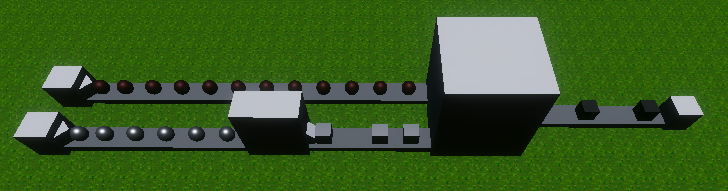
\includegraphics[scale=0.87]{Bilder/Stahl Fabrik.png}
\caption{Stahl Fabrik}
\label{fig:steel}
\end{figure}
Um zu sehen, welches Potential die datenorientierte Programmierung in der Spieleentwicklung bietet wurde eine Spielsimulation sowohl datenorientiert als auch objektorientiert erstellt. Das Spiel, welches simuliert und gemessen wird ist eine Art Aufbauspiel. Verglichen kann es mit dem populären Spiel \href{https://www.factorio.com/}{Factorio}. Hier wird es jedoch etwas schlichter und einfacher gehalten. Um beide Programmierparadigmen miteinander zu vergleichen wird eine kleine Fabrik in die Spielwelt generiert und vervielfältigt. Dies soll den Spieler simulieren. Die Fabrik ist abgebildet in Abbildung \ref{fig:steel}. Ganz links befinden sich zwei Kästen. Diese sollen Erzbohrer darstellen welche Eisenerz (silbern) und Kohle (braun) aus der Erde befördern und rechts auf ein Förderband legen. Die beiden Förderbänder transportieren die Kohle und das Eisenerz nach rechts weiter. Das Eisenerz wird als nächstes in Eisenbarren geschmolzen und sind deshalb rechteckig. Die Kohle und die Eisenbarren kommen dann gemeinsam in den großen Würfel, wo sie zu Stahl verarbeitet werden. Dieser Stahl wird dann wieder auf ein Förderband gelegt und in dem kleinen Würfel anschließend gelöscht. Die ganze Produktionskette soll möglichst einem Spiel nahekommen damit es eine möglichst realistische Simulation bietet und die Realität widerspiegelt. Nachfolgend wird gezeigt, wie die Spielsimulation möglichst ähnlich umgesetzt und gebenchmarkt wird.
\subsection{Objektorientierte Programmierung}
In der Objektorientierten Programmierung mit Unity dreht sich alles um GameObjects. Jedes Objekt in der Szene, egal ob sichtbar oder nicht ist ein GameObject. Diese GameObjects können verschiedene Komponenten haben, welche Eigenschaften definieren, also Daten speichern. Genauso haben diese Komponenten eine Start und eine Update Methode welche das Verhalten definieren. Die Start Methode wird einmalig vor dem ersten Aufruf der Update Methode ausgeführt. Die Update Methode läuft ein mal pro ausgegebenem Bild. Das Skript für eine Item sieht wie folgt aus:
\begin{lstlisting}[language={[Sharp]C}, caption={Item Component OOP}]
using Unity.Mathematics;
using UnityEngine;

public class Item : MonoBehaviour
{
    private int2 pos;
    [SerializeField] private int itemID;

    void Update()
    {
        transform.position = Vector3.Lerp(transform.position, new Vector3(pos.x, pos.y, -0.5f), Time.deltaTime * 2f);
    }

    public void SetPosition(int2 pos)
    {
        this.pos = pos;
    }

    public int GetItemID()
    {
        return itemID;
    }
}
\end{lstlisting}
Wie man sieht beinhaltet das MonoBehaviour nicht nur die Daten, sondern auch die Logik. Für ein Item benötigen wir zum einen die Position, wohin sich das Item bewegen soll, zum anderen speichern wir auch eine ID über die wir das Item ganz einfach identifizieren können. Das Attribut \glqq SerializeField\grqq{} zwingt Unity dazu ein editierbares Feld im Editor zu erstellen an dem man die itemID setzen kann. \ref{fig:SerializeField}
\begin{figure}
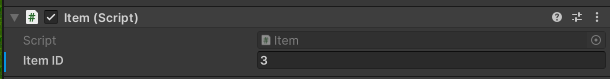
\includegraphics[scale=1]{Bilder/SerializeField.png}
\caption{SerializeField}
\label{fig:SerializeField}
\end{figure}
Eine Start Funktion ist in diesem Fall nicht notwendig. Die Update Methode bewegt das Item langsam an die übergebene Position. Time.deltaTime gibt die Zeit in Sekunden von dem letzten Bild bis zu dem momentanen Bild an. Dadurch wird die Bewegung linear.\\Ein weiterer Teil der Simulation ist die Bewegung der Items über das Förderband: 
\begin{lstlisting}[language={[Sharp]C}, caption={Förderband Component OOP}]
using System.Collections.Generic;
using UnityEngine;

namespace Buildings.Components
{
    public class BeltPath : MonoBehaviour
    {
        private List<ConveyorComponent> beltPath = new ();
        private InputConveyorComponent input;
        private OutputConveyorComponent output;
        private float timeToMove;

        public void Start()
        {
            input = GetComponent<InputConveyorComponent>();
            output = GetComponent<OutputConveyorComponent>();
            timeToMove = 2f;
        }

        public void Update()
        {
            timeToMove -= Time.deltaTime;
            if(timeToMove > 0) return;
            var lastBelt = beltPath[^1];
            if (!ReferenceEquals(lastBelt.item, null) && ReferenceEquals(output.GetItem(), null))
            {
                var item = lastBelt.item;
                var itemComponent = item.GetComponent<Item>();
                itemComponent.SetPosition(output.GetPosition());
                output.SetItem(item);
                lastBelt.item = null;
            }
            for (int i = beltPath.Count-2; i >= 0; i--)
            {
                var thisConveyor = beltPath[i];
                var lastConveyor = beltPath[i + 1];
                if (!ReferenceEquals(thisConveyor.item, null))
                {
                    if (ReferenceEquals(lastConveyor.item, null))
                    {
                        var item = thisConveyor.item;
                        var itemComponent = item.GetComponent<Item>();
                        lastConveyor.item = item;
                        itemComponent.SetPosition(lastConveyor.pos);
                        thisConveyor.item = null;
                    }
                }
            }
            var firstConveyor = beltPath[0];
            if (!ReferenceEquals(firstConveyor.item, null)) input.SetOccupied(true);
            else input.SetOccupied(false);
            if (!ReferenceEquals(input.GetItem(), null) && ReferenceEquals(firstConveyor.item, null))
            {
                firstConveyor.item = input.GetItem();
                input.RemoveItem();
            }
            timeToMove += 2f;
        }

        public void AddConveyor(ConveyorComponent conveyorComponent)
        {
            beltPath.Add(conveyorComponent);
        }
    }
}
\end{lstlisting}
Für das Förderband wird eine Liste mit vorhandenen Segmenten, der Input, der Output und eine Zeit gespeichert. Die Zeit wird in der Start Methode initialisiert und der Input bzw. Output wird über die Funktion \glqq GetComponent()\grqq{} von dem GameObject geholt. In der Update Funktion wird zunächst nur die timeToMove Variable herunter gezählt. Sollte diese Variable unter Null fallen, werden alle Items von hinten nach vorne ein Segment weiter bewegt sofern dies möglich ist. Ist der Output nicht belegt wird ein vorhandenes Item in den Output gelegt. Items auf den einzelnen Segmenten werden nach weiterbewegt und wenn ein Item im Input liegt wird dies auf das erste Segment weiterbewegt. Immer wenn ein Item weitergegeben wird (egal ob an ein Segment, oder an den Output) wird auch die neue Position an das Item weitergegeben. Durch das bewegen der Items von hinten nach vorne verhindert man, dass sich Items nicht bewegen, obwohl sie es könnten.
\subsection{Datenorientierte Programmierung}
In der datenorientierten Programmierung gehen wir statt der GameObjects auf die Komponenten und Systeme ein. Auch hier zu Beginn die Komponente für ein Item und das dazugehörige System:
\begin{lstlisting}[language={[Sharp]C}, caption={Item Component ECS}]
using Unity.Entities;
using Unity.Mathematics;

namespace ECS.Components
{
    public struct ItemComponent : IComponentData
    {
        public int2 pos;
        public int itemID;
    }
}
\end{lstlisting}
Auch hier wird die Position und die ID des Items gespeichert. Das dazugehörige System sieht ähnlich aus, wie das MonoBehaviour im Objektorientierten:
\begin{lstlisting}[language={[Sharp]C}, caption={Item System}]
using ECS.Components;
using Unity.Burst;
using UnityEngine;
using Unity.Entities;
using Unity.Transforms;

[BurstCompile(CompileSynchronously = true)]
public partial struct ItemSystem : ISystem
{
    
    [BurstCompile(CompileSynchronously = true)]
    public void OnUpdate(ref SystemState state)
    {
        new ItemMoveJob
        {
            deltaTime = SystemAPI.Time.DeltaTime
        }.ScheduleParallel();
    }

    [BurstCompile(CompileSynchronously = true)]
    public partial struct ItemMoveJob : IJobEntity
    {
        public float deltaTime;
        
        [BurstCompile(CompileSynchronously = true)]
        private void Execute(ref LocalTransform transform, in ItemComponent item)
        {
            transform = transform.WithPosition(Vector3.Lerp(transform.Position.xyz, new Vector3(item.pos.x, item.pos.y, -0.5f), deltaTime * 2f));
        }
    }
}
\end{lstlisting}
Jedoch sieht man hier schon Eigenheiten des Entity Component Systems, des Burst Compiler und dem Job System. Das Item System implementiert das Interface ISystem welches für unverwaltete Systeme verwendet werden muss. Zusätzlich ist die Struktur als auch deren Methoden und dem Job mit BurstCompile gekennzeichnet. Diese Kennzeichnung hilft dem Burst Compiler Methoden zu finden, welche mit Burst kompiliert werden sollen. Das Flag CompileSynchronously dient dem testen. Es besagt, dass erst das System durch den Burst Compiler kompiliert werden muss bevor es laufen kann. Andernfalls könnte das System schon laufen, ohne den Burst Compiler genutzt zu haben. Die Methode OnUpdate wird ein mal pro Bild aufgerufen. Sie ist zu vergleichen mit der Update Methode in einem MonoBehaviour. Innerhalb der OnUpdate Methode kommt das Job System von Unity zum Einsatz. Es wird der ItemMoveJob erstellt. Dieser Job funktioniert mit einem LocalTransform Component, welches jedes Entity besitzt und mit dem ItemComponent. Dabei wird das LocalTransform Component zum lesen und schreiben verwendet (erkennbar durch das Keywort ref) und das ItemComponent lediglich zum lesen (erkannbar durch das Keywort in). Auch hier wird nun die Position des Items mithilfe der Lerp Funktion von Vector3 und den Daten im ItemComponent verändert. Dieser Job, welcher die tatsächliche Logik für das Item enthält wird in der OnUpdate Methode parallel gescheduled. Dies ist hier speziell sehr vorteilhaft, da es sehr viele Items auf dem Spielfeld geben kann. Dadurch werden nicht tausende Items nacheinander bewegt, sondern alle zur gleichen Zeit.
\newpage
\section{Benchmark}
Auf die Erstellung der einzelnen Spielobjekte ist für den Benchmark nicht relevant. Es werden die Bilder pro Sekunde in Abhängigkeit von der Anzahl der Stahl Fabriken gezählt. 
\newpage
\section{Fazit}
\newpage
\section{Literaturverzeichnis}
\bibliographystyle{plain}
\bibliography{bibliography}

\newpage
\section{Anlagen}
\newpage
\section{Selbstständigkeitserklärung}
Ich, Dennis Untiet, erkläre, dass ich die vorliegende Arbeit selbstständig und nur unter Verwendung der
angegebenen Quellen und Hilfsmittel angefertigt habe.\\
Seitens des Verfassers bestehen Einwände die vorliegende Bachelorarbeit für die öffentliche Benutzung im
Universitätsarchiv zur Verfügung zu stellen.\\
Jena, \today, Unterschrift des Verfassenden
\end{document}